% Figure: t-SNE of ConvNeXt-Tiny pre-logit features, Task B test split
% Source   : artifact/person1/tsne/  (repo ManifoldsTeam/WoodID, branch p1,
%            commit d39a3f6b2cc5942e1e718c0dca86e89b0d81eb4d; see SOURCE.txt)
% Run id   : taskB17__main__seed_42__convnext_tiny  (same registry as Table 1)
% Artifacts: features_convnext_seed42_test.npz, tsne_embedding.csv,
%            tsne_metadata.json
\begin{figure}[!htbp]
\centering
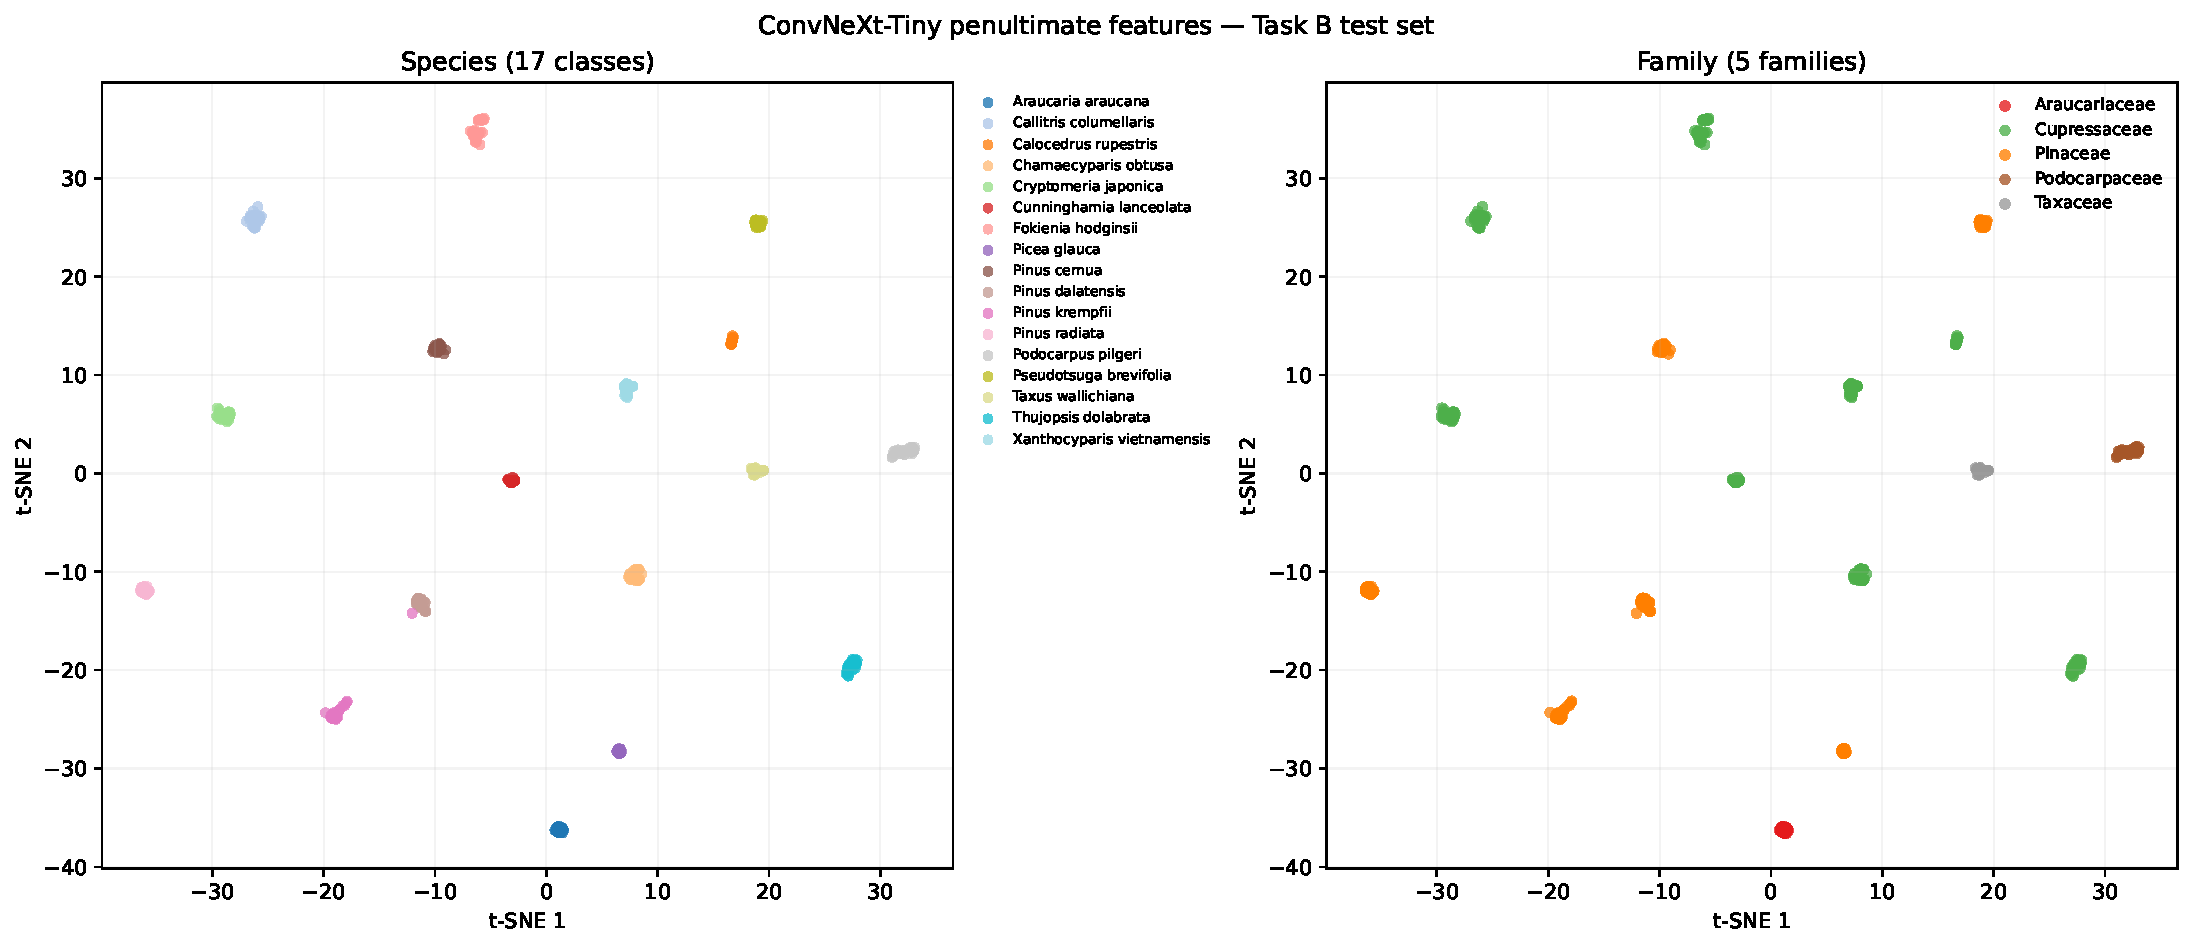
\includegraphics[width=\linewidth]{artifact/person1/tsne/fig_tsne.pdf}
\caption{Two-dimensional t-SNE embedding of ConvNeXt-Tiny features for all 532
Task~B test images, taken from the seed-42 run of
Table~\ref{tab:task_b}. Features are the 768-dimensional pre-logit activations,
standardised, reduced to 50 dimensions by PCA and then to two by t-SNE with
perplexity 30, PCA initialisation and a fixed random seed. t-SNE preserves
local neighbourhoods only: distances and cluster areas in the plot are not
metric, and the embedding is shown as a qualitative view of the representation
rather than as evidence of separability.}
\label{fig:tsne}
\end{figure}
